\documentclass[a4paper,11pt]{article}

\usepackage{préambule}

\TitreDActivite{Activité : Fractions sur une droite}

\newcommand{\DessineCorrection}{0}
\ifthenelse{\DessineCorrection=1}{
	\renewcommand{\phantom}[1]{{#1}}
}

\begin{document}

\maketitle

\begin{exercice}\

	Écrit la fraction $\dfrac{3}{4}$ sous forme de nombre décimal (nombre à virgule) : .............. \phantom{\color{red} 0,75}

	\vspace{0.4em}

	Place la fraction $\dfrac{3}{4}$ sur la droite graduée :

	\begin{center}
		\begin{tikzpicture}[scale=10]
			\draw[thick,->] (-0.1,0) -- (1.1,0);
			\foreach \x in {0,0.25,0.5,0.75,1} {
					\draw[thick] (\x,0) -- (\x,-0.02) node[below] {\x};
				}
			\node[red] at (3 / 4, 0) {\phantom{×}};
			\node[red,above] at (3 / 4, 0) {\phantom{$\dfrac{3}{4}$}};
		\end{tikzpicture}
	\end{center}

	Place les fractions $\dfrac{8}{2}$, $\dfrac{27}{9}$, $\dfrac{15}{6}$ et $\dfrac{12}{16}$ sur la droite graduée :

	\begin{center}
		\begin{tikzpicture}[scale=2]
			\draw[thick,->] (-0.5,0) -- (5.5,0);
			\foreach \x in {0,...,5} {
					\draw[thick] (\x,0) -- (\x,-0.1) node[below] {\x};
				}
			\foreach \a/\b in {8/2,27/9,15/6,12/16} {
					\node[red] at (\a / \b, 0) {\phantom{×}};
					\node[red,above] at (\a / \b, 0) {\phantom{$\dfrac{\a}{\b}$}};
				}
		\end{tikzpicture}
	\end{center}

	La fraction $\dfrac{8}{2}$ est-elle plus petite que $\dfrac{27}{9}$ ? \phantom{\color{red} Non}

	Range les quatre fractions dans l'ordre croissant :

	\dotfill\phantom{\color{red} $\dfrac{12}{16} < \dfrac{15}{6} < \dfrac{27}{9} < \dfrac{8}{2}$}

\end{exercice}

\begin{exercice}\

	\begin{enumerate}
		\item Avec une règle graduée, dessine un rectangle de 16cm de largeur et 1cm de hauteur. Puis, partage ce rectangle en 8 parties égales.

		      \begin{center}
			      \phantom{
				      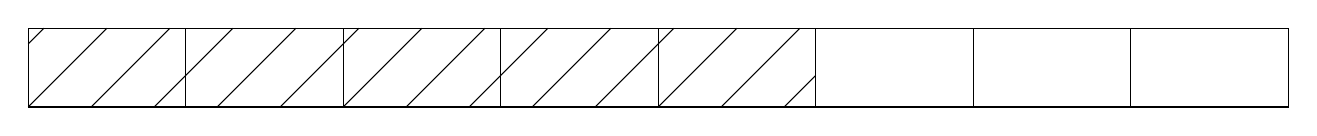
\begin{tikzpicture}
					      \draw (0,0) rectangle (16,1);
					      \foreach \x in {1,...,7} {
							      \draw (\x / 8 * 16, 0) -- ++(0, 1);
						      }
					      \foreach \x in {0,...,11} {
							      \draw (\x / 1.25, 0) -- (\x / 1.25 + 1, 1);
						      }
					      \draw (0,0.8) -- (0.2, 1);
					      \draw (9.6,0) -- (10, 0.4);
				      \end{tikzpicture}
			      }
		      \end{center}

		      Hachure les 5 premières parties ( comme ceci: \tikz{
			      \draw (0,0) rectangle (1,0.35);
			      \draw (0,0.3) -- (0.05,0.35);
			      \draw (0,0) -- (0.35,0.35);
			      \draw (0.3,0) -- (0.65,0.35);
			      \draw (0.6,0) -- (0.95,0.35);
			      \draw (0.9,0) -- (1,0.1);
		      } ).

		      Quelle fraction représente la partie hachurée ? ............. \phantom{\color{red} $\dfrac{5}{8}$}

		\item Sur la droite graduée suivante, place :

		      \begin{enumerate}
			      \item La fraction $\dfrac{8}{8}$, à l'endroit de ton choix.
			      \item La fraction $\dfrac{5}{8}$.
		      \end{enumerate}

		      \begin{center}
			      \begin{tikzpicture}[scale=10]
				      \draw[thick,->] (-0.05,0) -- (1.05,0);
				      \draw (0,0) -- (0,-0.02) node[below] {0};
				      \node[red] at (8 / 8, 0) {\phantom{×}};
				      \node[red,above] at (8 / 8, 0) {\phantom{$\dfrac{8}{8}$}};
				      \node[red] at (5 / 8, 0) {\phantom{×}};
				      \node[red,above] at (5 / 8, 0) {\phantom{$\dfrac{5}{8}$}};
			      \end{tikzpicture}
		      \end{center}

		\item Place les fractions $\dfrac{1}{3}$, $\dfrac{5}{3}$, $\dfrac{3}{2}$ et $\dfrac{5}{4}$ sur la droite graduée :

		      \begin{center}
			      \begin{tikzpicture}[scale=5]
				      \draw[thick,->] (-0.1,0) -- (3.1,0);
				      \foreach \x in {0,0.5,1,1.5,2,2.5,3} {
						      \draw[thick] (\x,0) -- (\x,-0.04) node[below] {\x};
					      }
				      \foreach \a/\b in {1/3,5/3,3/2,5/4} {
						      \node[red] at (\a / \b, 0) {\phantom{×}};
						      \node[red,above] at (\a / \b, 0) {\phantom{$\dfrac{\a}{\b}$}};
					      }
			      \end{tikzpicture}
		      \end{center}
	\end{enumerate}

	Range les quatre fractions dans l'ordre croissant :

	\dotfill\phantom{\color{red} $\dfrac{1}{3} < \dfrac{5}{4} < \dfrac{3}{2} < \dfrac{5}{3}$}
\end{exercice}

\end{document}